\section{Relative Error and Graphic Analysis}
\label{sec:erroranalysis}

\subsection{Frequency Responde Analysis}
\label{subsec:freqresp}

\begin{figure}[H]

\begin{subfigure}{0.5\textwidth}
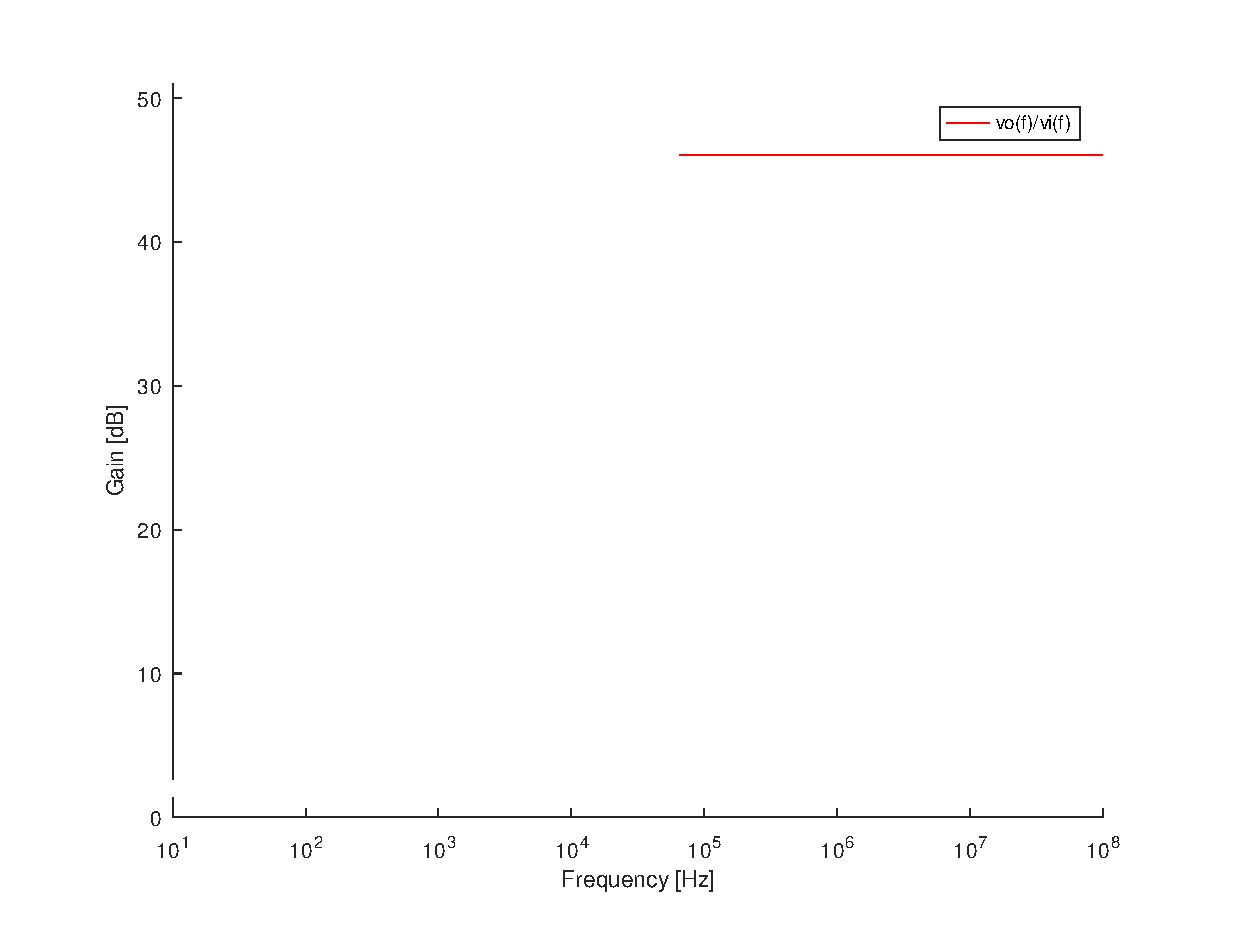
\includegraphics[width=0.9\linewidth, height=8cm]{gain.eps} 
\caption{Phase of $v_s(f)$,  $v_c(f)$  and $v_6(f)$ during frequency interval [0.1 , 1] MHz, obtained using GNU Octave.}
\label{fig:theo_third}
\end{subfigure}
\begin{subfigure}{0.5\textwidth}
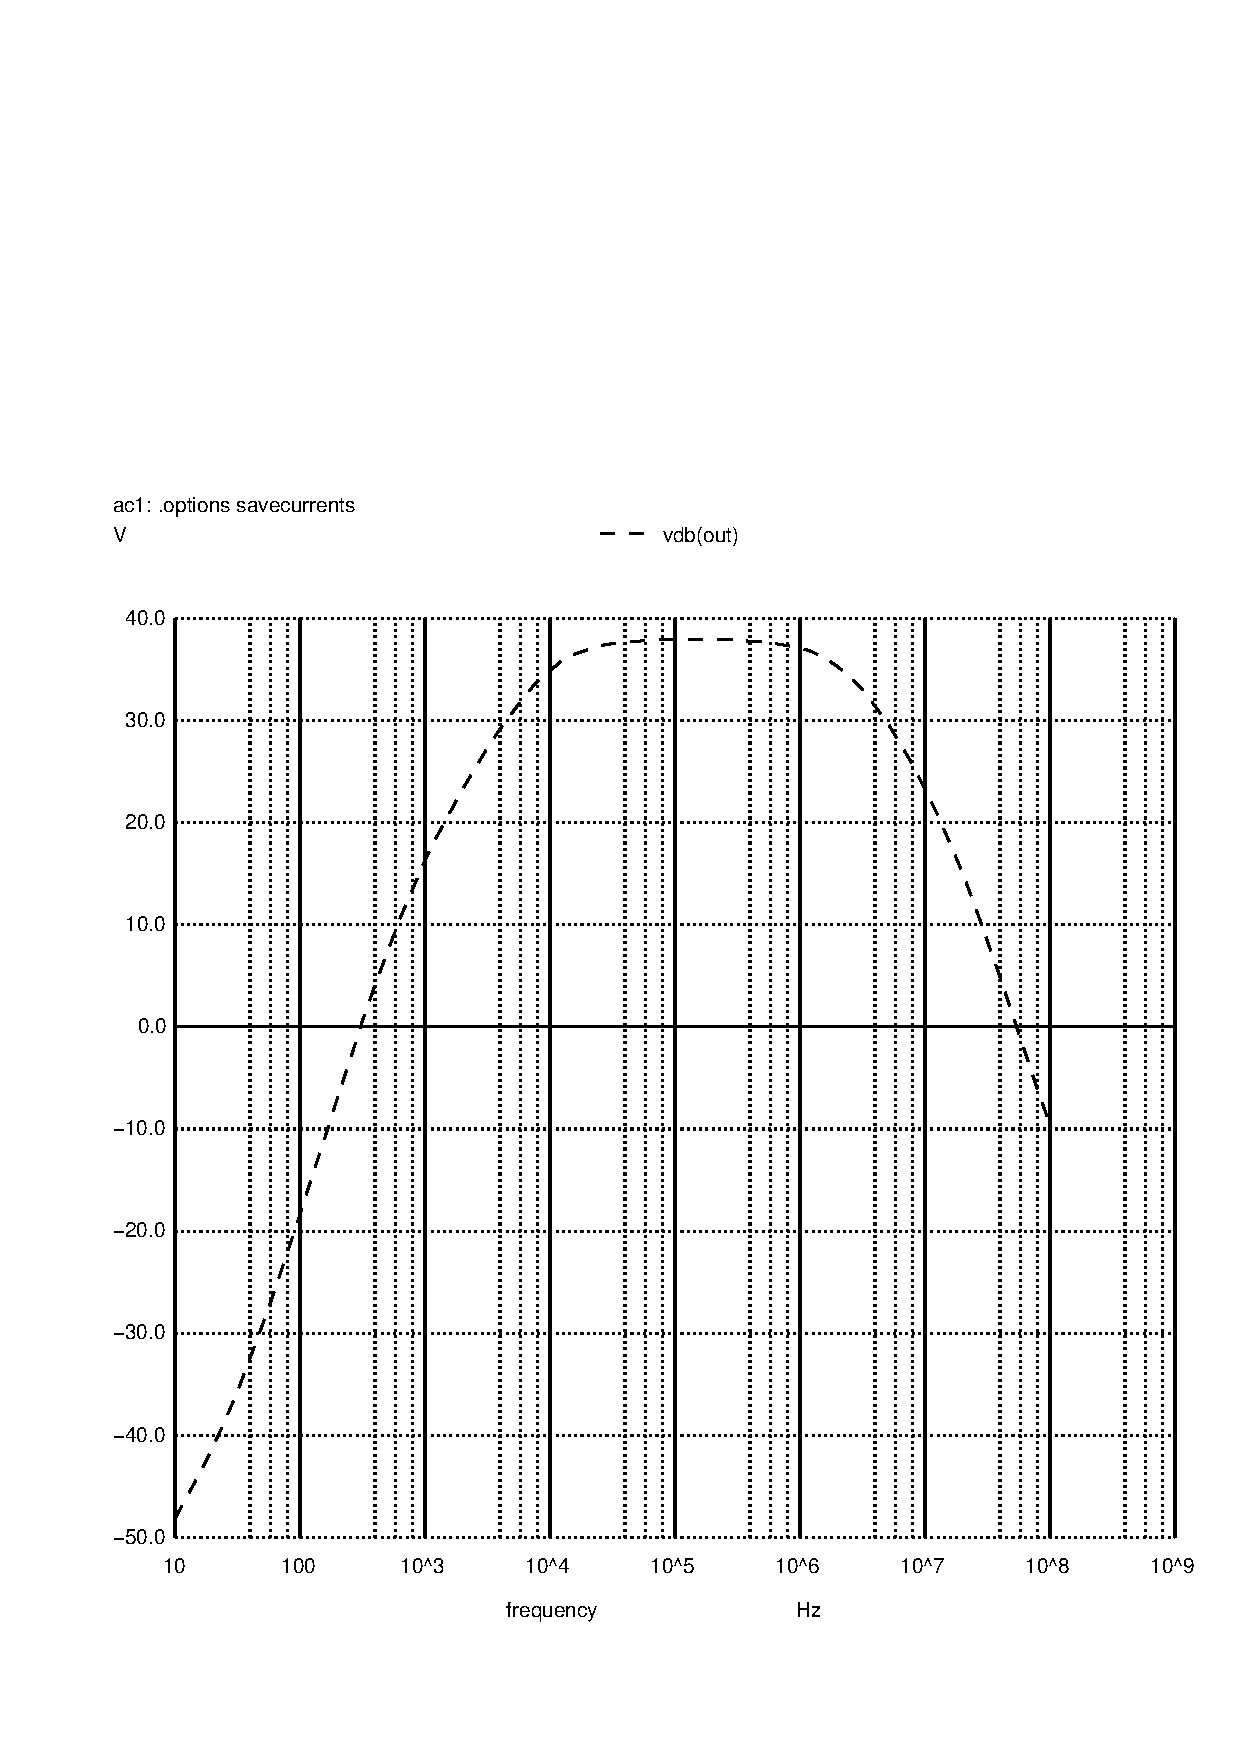
\includegraphics[width=0.8\linewidth, height=8cm]{vo2f.pdf}
\caption{Phase of $v_s(f)$ and $v_6(f)$ during frequency interval [0.1 , 1] MHz, obtained using Ngspice.}
\label{fig:total}
\end{subfigure}
\end{figure}

\subsection{Input and Output Impedances Analysis}
\label{subsec:freqresp}

\begin{center}
   \begin{table}[H]
\resizebox{\textwidth}{!}{%
\begin{tabular}{cc|c|c|c|c|}
\cline{3-6}
\multicolumn{2}{c}{} & \textbf{NGSpice Value} & \textbf{Octave Value} & \textbf{Relative Error} & \textbf{Percentual Error {[}\%{]}} \\ \hline
\multicolumn{1}{|c|}{\multirow{2}{*}{Gain Stage}} & Input Impedance & 574.5327 & 523.575168 & 0.08869387591 & 8.869387591 \\ \cline{2-6} 
\multicolumn{1}{|c|}{} & Output Impedance & 799.9195 & 730.963158 & 0.08620410179 & 8.620410179 \\ \hline
\multicolumn{1}{|c|}{\multirow{2}{*}{Output Stage}} & Input Impedance & 65771.74 & 78634.69849 & 0.1955696852 & 19.55696852 \\ \cline{2-6} 
\multicolumn{1}{|c|}{} & Output Impedance & 3.17595 & 3.171596 & 0.001370928384 & 0.1370928384 \\ \hline
\multicolumn{1}{c|}{} & Voltage Gain & 37.93 & 46.02225 & 0.2133469549 & 21.33469549 \\ \cline{2-6} 
\end{tabular}%
}
\end{table}
 \end{center}

\paragraph{}
In the table above, we have the comparison between Octave and NGSpice of the Output Voltage Gain, the Input Impedance and the Output Impedance. The percentual error is also included to make the interpretation easier. As we can see, the percentual relative errors presented are very high and thus cannot be ignored. A possible explanation for these discrepancies is that NGSpice uses a very complex transistor model, similarly to what happened in the previous laboratory assignment with the diode model, which does not have fixed parameters, and so it becames very hard for Octave to match the results.

\subsection{Figure of Merit}
\label{subsec:Figure_of_Merit}


\paragraph{}
To end our report, we present the figure of merit. It is important to remind that this figure is obtained upon the devices and values used in Ngspice. During our work, we have performed several incremental modifications to improve the merit figure. It was really important for us to understand the influence of the coupling capacitors on the bandwidth, the purpose of the bypass capacitor in relation with the voltage gain and the effect of resistors and capacitors. 

\paragraph{}
The variation of these parameters allowed us to achieve an improved figure of merit, while trying to maximize the voltage gain and the bandwith and to minimize the cost of the circuit' components and to achieve the lowest lower cut-off frequency as posible. The values applied both in NGSpice and Octave proved to be our best options to make the figure of merit as high as possible.
